\documentclass[12pt]{article}
\usepackage{geometry}                % See geometry.pdf to learn the layout options. There are lots.
\geometry{letterpaper}                   % ... or a4paper or a5paper or ... 
%\geometry{landscape}                % Activate for for rotated page geometry
\usepackage[parfill]{parskip}    % Activate to begin paragraphs with an empty line rather than an indent
\usepackage{daves,fancyhdr,natbib,graphicx,dcolumn,amsmath,lastpage,url}
\usepackage{amsmath,amssymb,epstopdf,longtable}
\usepackage[final]{pdfpages}
\DeclareGraphicsRule{.tif}{png}{.png}{`convert #1 `dirname #1`/`basename #1 .tif`.png}
\pagestyle{fancy}
\lhead{CE 5364 -- Groundwater Transport Phenomena }
\rhead{FALL 2024}
\lfoot{ES5}
\cfoot{}
\rfoot{Page \thepage\ of \pageref{LastPage}}
\renewcommand\headrulewidth{0pt}



\begin{document}
\begin{center}
{\textbf{{ CE 5364 Groundwater Transport Phenomena } \\ {Exercise Set 5}}}
\end{center}

\section*{\small{Exercises}}
\begin{enumerate} %% Problem Counter

%%%%%%%%%%%%%%%%%%%%%%%%%%%%%%%%%%%%%%%%%%%%%%%%%%%%

\item (Problem 11-1, pg. 594)

A contaminated site has been surveyed and a contaminated region $100~ft. \times 150~ft. \times 15~ft.$ was delineated. The average concentration of total petroleum hydrocarbons (TPH) in soil is $10,000~\frac{mg}{Kg}$

Determine:

\begin{enumerate} %% Deliverable Counter
\item The total mass of contaminants at the site in kilograms. Assume the soil has a specific gravity, $SG _{soil} \approx 2.0$
\item Estimate total volume of petroleum hydrocarbons released assuming 50% of the hydrocarbins are lost to volatization, biodegredation, and dissolution (report the answer in gallons). Assume the hydrocarbons were gasoline with a constant specific gravity, $SG_{\text{gasoline}} \approx 0.8$
\item Estimate the residual saturation of the hydrocarbon-soil system.  Assume soil porosity is, $n=0.35$
\end{enumerate} %% Deliverable Counter



\clearpage

%%%%%%%%%%%%%%%%%%%%%%%%%%%%%%%%%%%%%%%%%%%%%%%%%%%%%%%%%%
\item (Problem 11-2, pg. 594)
A sampling program at a Supermanfund site indicated the following DNAPL zones:
\begin{itemize}
\item A pool of free phase DNAPL in a stratigraphic depression in an unfractured clay. The pool is 200 $ft^2$ in area and 5 $ft$ thick.
\item A zone of residual DNAPL extending directly underneath an old disposal pit 100 $ft^2$ in area.  The residual zone extends through the 5 $ft$ thick unsaturated zone and 15 $ft$ through the saturated zone until it reaches the DNAPL pool.
\end{itemize}

\begin{figure}[h!] %  figure placement: here, top, bottom, or page
   \centering
   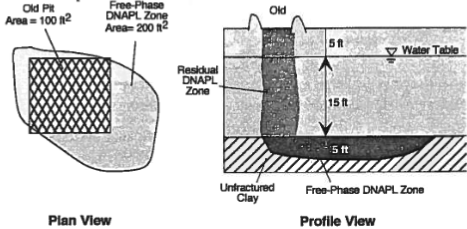
\includegraphics[width=6.5in]{pr2.1.png} 
   \caption{Schematic of Contamination Scenario}
   \label{fig:profileplot}
\end{figure}

\begin{table}[htbp]
\centering
\caption{Supporting Data}
\begin{tabular}{p{3.5in}p{1.5in}} % Column formatting, @{} suppresses leading/trailing space
~&~\\
Item & Value \\
Residual saturation in the unsaturated zone: & 0.10\\
Residual saturation in the saturated zone: & 0.35\\
Saturation in the free-phase zone: & 0.70\\
Average porosity in water zone: & 0.30\\
\end{tabular}
\label{tab:supporting}
\end{table}

\newpage

Determine:
\begin{enumerate} %% Deliverable Counter
\item The total volume of DNAPL at the site
\item The recoverable volume using ordinary pumping.
\end{enumerate} %% Deliverable Counter
\clearpage
%%%%%%%%%%%%%%%%%%%%%%%%%%%%%%%%%%%%%%%%%%%%%%%%%%%%%%
%%%%%%%%%%%%%%%%%%%%%%%%%%%%%%%%%%%%%%%%%%%%%%%%%%%%%%
\item (Problem 11-4, pg. 595)

Gasoline is found in a monitoring well with $SG=0.80$.  A total depth of 6 $ft$ of gasoline is found in the well.

Determine:
\begin{enumerate} %% Deliverable Counter
\item Estimated thickness of free-phase LNAPL in the formation.
\end{enumerate} %% Deliverable Counter

%%%%%%%%%%%%%%%%%%%%%%%%%%%%%%%%%%%%%%%%%%%%%%%%%%%%%%%%%%%%%%%%%%%
\end{enumerate}%% Problem Counter

\end{document}  